\subsection{Digital, discretized PLL Model}
Based on the continuous PLL theory, a model for digital, discretized PLLs (i.e. ADPLLs) can be adapted. The general approach here is to utilize the bilinear transformation between continuous s-domain models to the discrete z-domain models. As commonly cited in PLL literature from a seminal paper by Gardner \cite{gardner_1980}, if the sampling frequency $f_s > 10\cdot\textnormal{BW}_{loop}$, where BW$_{loop}$ is the PLL loop bandwidth, the effects of time sampling are easily ignored for purposes of analysis. Thus the design methods established in this paper are predicated on $f_s > 10\cdot\textnormal{BW}_{loop}$.
\begin{figure}[htb!]
	\center\fontfamily{\sfdefault}\selectfont
% XCircuit output "basic_adpll.tex" for LaTeX input from basic_adpll.ps
\def\putbox#1#2#3#4{\makebox[0.00000in][l]{\makebox[#1][l]{}\raisebox{\baselineskip}[0.00000in][0.00000in]{\raisebox{#2}[0.00000in][0.00000in]{\scalebox{#3}{#4}}}}}
\def\rightbox#1{\makebox[0.00000in][r]{#1}}
\def\centbox#1{\makebox[0.00000in]{#1}}
\def\topbox#1{\raisebox{-0.60\baselineskip}[0.00000in][0.00000in]{#1}}
\def\midbox#1{\raisebox{-0.20\baselineskip}[0.00000in][0.00000in]{#1}}
   \scalebox{1}{
   \normalsize
   \parbox{5.07500in}{
   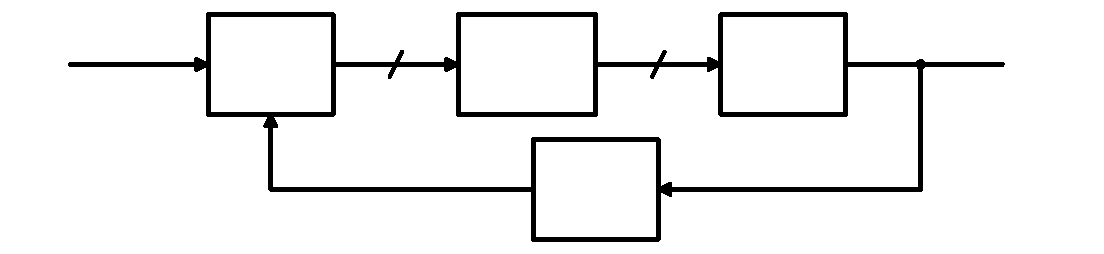
\includegraphics[scale=0.70000]{./figs/basic_adpll.pdf}\\
   % translate x=368 y=488 scale 0.38
   \putbox{1.09200in}{0.82600in}{1.20}{TDC}%
   \putbox{2.63200in}{0.24500in}{1.20}{$\div$ N}%
   \putbox{0.35700in}{0.97300in}{1.20}{$\Phi_{ref}$[n]}%
   \putbox{4.09500in}{0.97300in}{1.20}{$\Phi_{out}$[n]}%
   \putbox{2.19800in}{0.82600in}{1.20}{H$_{LF}$(z)}%
   \putbox{3.47900in}{0.82600in}{1.20}{DCO}%
   \putbox{1.67300in}{0.39200in}{1.20}{$\Phi_{div}$[n]}%
   \putbox{1.64500in}{1.02900in}{1.20}{e$_{\Phi}$[n]}%
   \putbox{2.92600in}{1.02900in}{1.20}{u[n]}%
   } % close 'parbox'
   } % close 'scalebox'
   \vspace{-\baselineskip} % this is not necessary, but looks better
\fontfamily{\rmdefault}\selectfont

	\caption{Basic ADPLL.}
	\label{fig:basic_adpll}
\end{figure}
\FloatBarrier
The basic architecture of an ADPLL is shown in figure \ref{fig:basic_adpll}. Here, compared to the continuous PLL, the phase detector has been replaced with a time to digital converter (TDC), the loop filter $\mathrm{H}_{LF}(s)$ with a discrete loop filter $\mathrm{H}_{LF}(z)$, and the VCO with a digitally controlled oscillator (DCO). In this architecture, the TDC, loop filter, and DCO are digital. 

\subsubsection{Divider}
A digital divider behaves nearly identical to the continuous case:
\begin{equation}
	\Phi_{div}[n] = \frac{\Phi_{out}[n]}{\mathrm{N}}
\end{equation}
Application of the z-transfrom:
\begin{equation}
	\frac{\Phi_{div}(z)}{\Phi_{out}(z)} = \frac{1}{\mathrm{N}}
\end{equation}
\subsubsection{TDC}
The TDC is a digital, quantized representation of the the phase detector. It takes input phase signals $\Phi_{div}$[n] and $\Phi_{ref}$[n], and outputs a digital phase error measurement word $e_\Phi[n]$. Figure \ref{fig:tdc} shows the basic TDC model architecture. A TDC will have limited resolution in phase, equivalent to M steps per reference cycle. This is a minimum step size in time of $\Delta t_{step}$ = $1/Mf_{ref}$. Since the output of the TDC is digital, the model applies a scale factor M$/2\pi$ and floor rounding, so 1 LSB of $e_\Phi[n]$ equates to $\Delta t_{step}$ timing error  between $\Phi_{div}$[n] and $\Phi_{ref}$[n].
\begin{figure}[htb!]
	\center\include{./figs/tdc}
	\caption{TDC model.}
	\label{fig:tdc}
\end{figure}
\begin{equation}
	e_\Phi[n] = \left\lfloor\frac{\mathrm{M}}{2\pi}(\Phi_{ref}[n] - \Phi_{div}[n])\right\rfloor
\end{equation}
For purposes of PLL transfer function calculation, the z-domain representation is as follows. Effects of quantization will be handled in section \ref{pn_theory}.
\begin{equation}
	e_\Phi(z) = \frac{\mathrm{M}}{2\pi}(\Phi_{ref}(z) - \Phi_{div}(z))
\end{equation}	
\FloatBarrier
\subsubsection{Loop Filter}
The loop filter design will be derived from the continuous PI-controller loop filter with optional peaking compensation (equation \ref{eq:pi_compensated_tf}) via application of the bilinear transform. The bilinear transform specifically allows for the conversion of a continuous transfer function to discrete representation, and vice versa. This, however is conditioned on satisfaction of Nyquist sampling criteria, and in the case of PLLs it is recommended that $f_s > 10\cdot\mathrm{BW}_{loop}$ to ensure transformation accuracy \cite{gardner_1980}. A high level of oversampling allows for the following definition of the bilinear transform, where 1/T=$f_{ref}$:
\begin{align*}
	z^{-1} &= e^{-sT} && \text{(definition of z-space)} \\
	&= \sum_{k=0}^\infty\frac{(-sT)^k}{k!} && \text{(exponential Taylor series)} \\
	&\approx 1-sT &&\text{(if $|sT| = 2\pi\mathrm{BW}_{loop}\cdot T << 1$)} \\
\end{align*}
Thus the bilinear transform identities are:
\begin{align}
	z^{-1} &= 1-sT\\
	s &= \frac{1}{T}(1-z^{-1}) \label{eq:s_to_z}
\end{align}
Applying \ref{eq:s_to_z} to equation \ref{eq:pi_compensated_tf} yields the z-domain loop filter:
\begin{align}
	\textnormal{H}_{LF}(z) = \left.\textnormal{H}_{LF}(s)\right\vert_{s=\frac{1}{T}(1-z^{-1})} = \left.\frac{K_i}{s}\frac{\left(\frac{s}{\omega_z} + 1\right)}{\left(\frac{s}{\omega_p} + 1\right)}\right\vert_{s=\frac{1}{T}(1-z^{-1})}\\
	= \frac{\omega_p}{\omega_z}\frac{k_iT}{(1-z^{-1})}\frac{(1+\omega_zT)-z^{-1}}{(1+\omega_pT) - z^{-1}(2+\omega_pT) + z^{-2}}\label{eq:z_lf}
\end{align}
Equation \ref{eq:z_lf} is converted to a digitally implementable representation via converting into the canonical representation of \ref{eq:canonical_z}, which determines the tap coefficients for the sampled-time difference equation \ref{eq:cananical_diff}. 
\begin{align}
	\textnormal{H}_{LF}(z) &= \frac{\sum_{j=0}^M b_jz^{-j}}{1+\sum_{k=1}^N a_kz^{-k}}\label{eq:canonical_z} \\
	y[n]&= -\sum_{k=1}^N a_ky[n-k] + \sum_{j=0}^M b_jx[n-j] \label{eq:cananical_diff}
\end{align}
Equation \ref{eq:cananical_diff} is directly implementable in digital hardware with a direct type 1 IIR filter shown in figure \ref{fig:filt_imple}, with the filter coefficients given by equations \ref{eq:a1}-\ref{eq:b1}. The filter coefficients must be quantized into finite resolution fixed point words for a complete digital implementation. Effects of quantization will be discussed in section \ref{pn_theory}.
\begin{figure}[htb!]
	\center\fontfamily{\sfdefault}\selectfont
% XCircuit output "filter_arch_tex.tex" for LaTeX input from filter_arch_tex.ps
\def\putbox#1#2#3#4{\makebox[0.00000in][l]{\makebox[#1][l]{}\raisebox{\baselineskip}[0.00000in][0.00000in]{\raisebox{#2}[0.00000in][0.00000in]{\scalebox{#3}{#4}}}}}
\def\rightbox#1{\makebox[0.00000in][r]{#1}}
\def\centbox#1{\makebox[0.00000in]{#1}}
\def\topbox#1{\raisebox{-0.60\baselineskip}[0.00000in][0.00000in]{#1}}
\def\midbox#1{\raisebox{-0.20\baselineskip}[0.00000in][0.00000in]{#1}}
   \scalebox{1}{
   \normalsize
   \parbox{5.54167in}{
   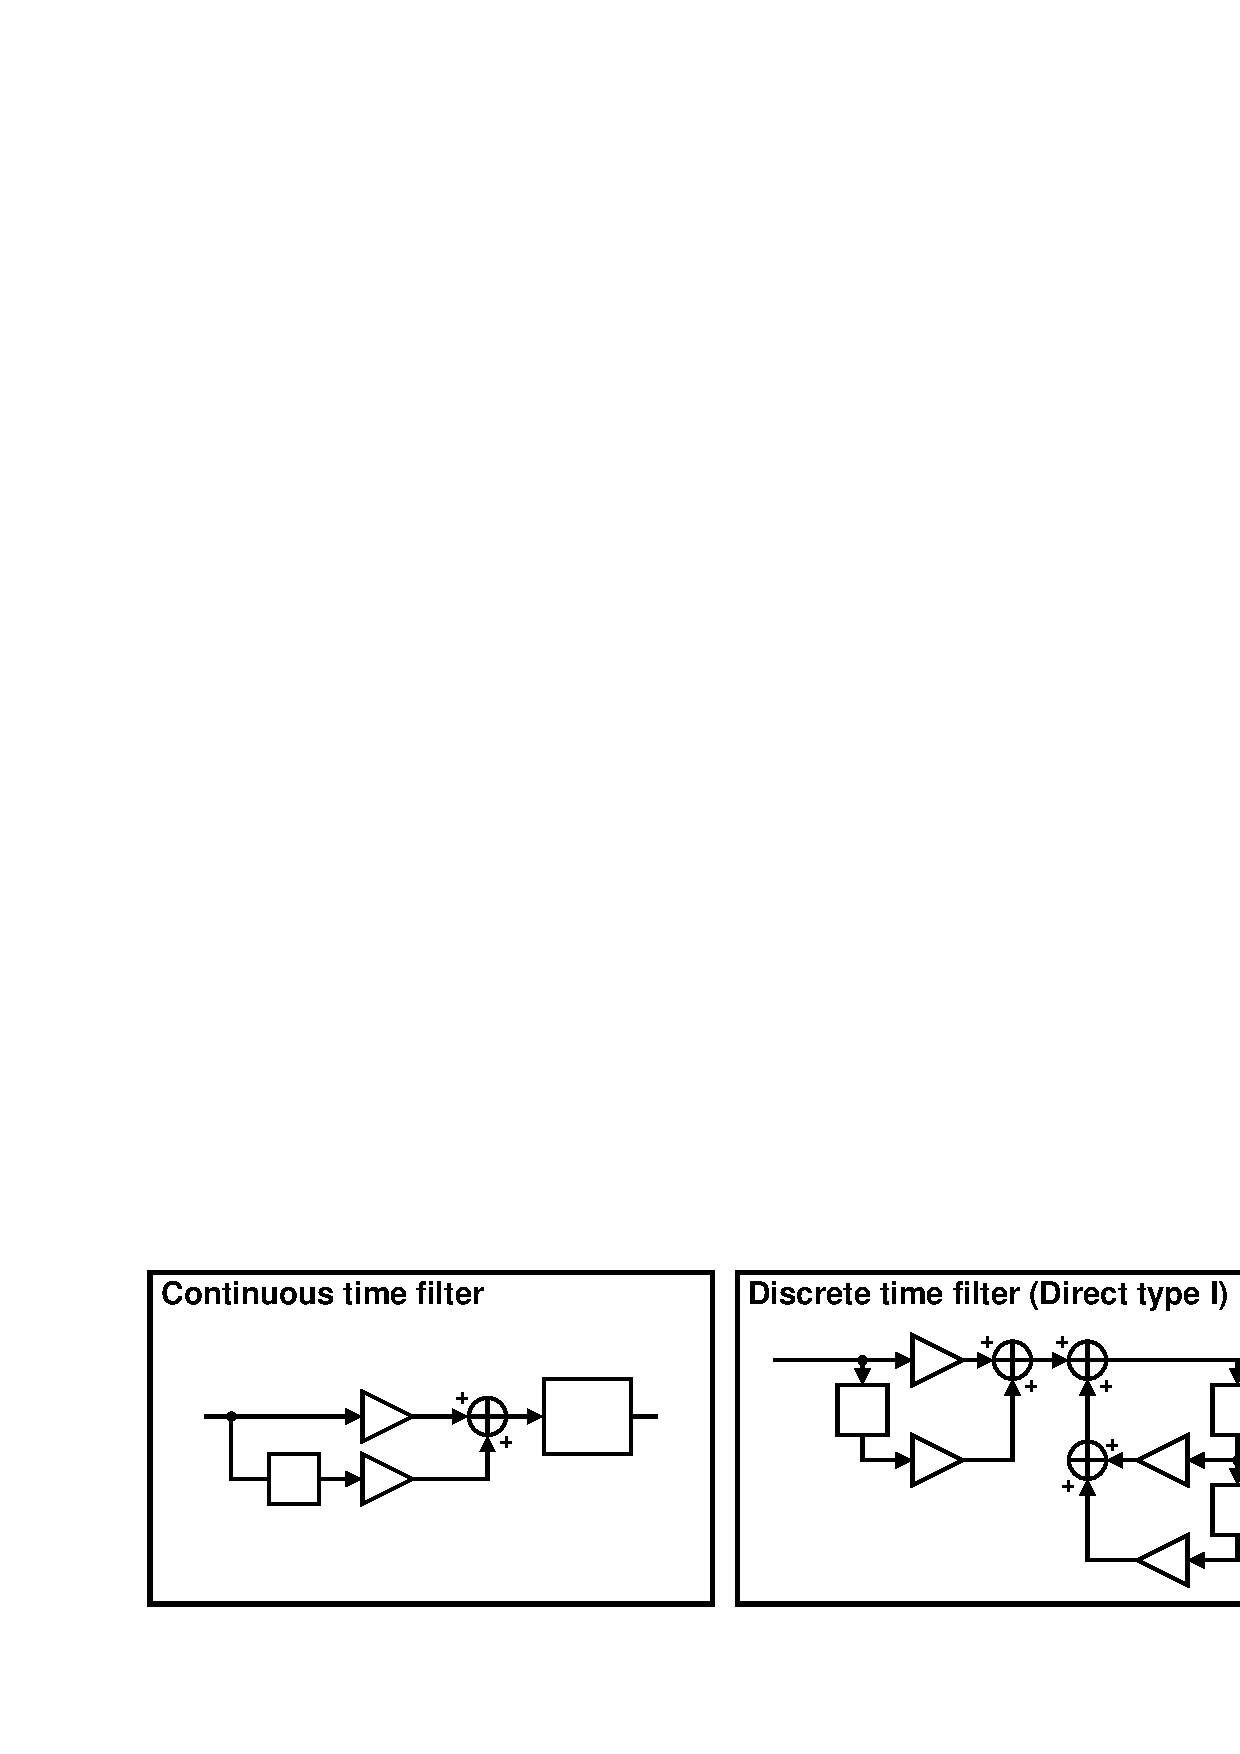
\includegraphics[scale=0.70000]{./figs/filter_arch_tex.pdf}\\
   % translate x=1728 y=944 scale 0.38
   \putbox{1.91800in}{0.90300in}{0.96}{$\frac{1}{\frac{s}{\omega_p} + 1}$}%
   \putbox{1.14800in}{1.01500in}{0.96}{$K_p$}%
   \putbox{1.14800in}{0.72800in}{0.96}{$K_i$}%
   \putbox{0.60900in}{0.58100in}{0.96}{$1/s$}%
   \putbox{0.25900in}{0.98700in}{0.96}{x[n]}%
   \putbox{2.35900in}{0.98700in}{0.96}{y[n]}%
   \putbox{2.92600in}{1.25300in}{0.96}{x[n]}%
   \putbox{5.17300in}{1.16200in}{0.96}{y[n]}%
   \putbox{3.26200in}{0.90300in}{0.96}{$z^{-1}$}%
   \putbox{3.73100in}{1.28100in}{0.96}{b$_0$}%
   \putbox{3.73100in}{0.81200in}{0.96}{b$_1$}%
   \putbox{5.01200in}{0.90300in}{0.96}{$z^{-1}$}%
   \putbox{5.01200in}{0.43400in}{0.96}{$z^{-1}$}%
   \putbox{4.60600in}{0.82600in}{0.96}{-a$_1$}%
   \putbox{4.59200in}{0.35700in}{0.96}{-a$_2$}%
   \putbox{5.17300in}{0.69300in}{0.96}{y[n-1]}%
   \putbox{5.15900in}{0.23100in}{0.96}{y[n-2]}%
   } % close 'parbox'
   } % close 'scalebox'
   \vspace{-\baselineskip} % this is not necessary, but looks better
\fontfamily{\rmdefault}\selectfont

	\caption{Implementation of filter.}
	\label{fig:filt_imple}
\end{figure}
			% y[n] = x[n]\frac{K_i\omega_pT}{\omega_z}\frac{1+\omega_zT}{1+\omega_pT} - x[n-1]\frac{K_i\omega_pT}{\omega_z}\frac{1}{1+\omega_pT} + y[n-1]\frac{2+\omega_pT}{1+\omega_pT} - y[n-2]\frac{1}{1+\omega_pT}\\
			% = a_0x[n] + a_1x[n-1] - b_1y[n-1] - b_2x[n-2] 
\begin{align}
	a_1 &= -\frac{2+\omega_pT}{1+\omega_pT}\label{eq:a1}\\
	a_2 &= \frac{1}{1+\omega_pT} \\
	b_0 &= \frac{K_i\omega_pT}{\omega_z}\frac{1+\omega_zT}{1+\omega_pT}\\
	b_1 &= \frac{K_i\omega_pT}{\omega_z}\frac{1}{1+\omega_pT}\label{eq:b1}
\end{align}
\subsubsection{DCO}
The DCO is modeled in discrete time as a recursive phase integrator, dependent on the DCO gain $K_{DCO}$, which provides the frequency tuning per LSB of the oscillator, the input oscillator tuning word u[n], and the sampling period T.
\begin{equation}
	\Phi_{out}[n] = \Phi_{out}[n-1] + 2\pi K_{DCO}u[n]T
\end{equation}
Application of the z-transform yields:
\begin{equation}
	\frac{\Phi_{out}(z)}{u(z)} = \frac{2\pi K_{DCO}T}{1-z^{-1}}
\end{equation}
Application of the bilinear transform to the DCO transfer function yields:
\begin{equation}
	\frac{\Phi_{out}(s)}{u(s)} = \frac{2\pi K_{DCO}T}{1-(1-sT)} = \frac{2\pi K_{DCO}}{s} 
\end{equation}
\subsubsection{Discrete-time PLL transfer function}
The transfer function for the discrete-time PLL can be computed in the z-domain, and also approximated continuously. The open loop z-domain transfer function is:

\subsection{PLL Noise} \label{pn_theory}
fasf
Generic theory of PLL
Discrete PLL
Noise theory
